
	\documentclass{article}
	\usepackage{amsmath,amssymb}
	\usepackage[inline]{enumitem}
	\usepackage{blindtext}
	\usepackage{booktabs}
	\usepackage{graphicx}
	\usepackage{xcolor}
	\usepackage[vmargin = 1.5in, top = 1in, bottom = 1.2in, letterpaper]{geometry}
	\usepackage{listings}
	\usepackage{courier}
	\lstset{
	basicstyle = \small\tt,
	keywordstyle = \tt\color{blue},
	commentstyle = \it\color[cmyk]{1,0,1,0},
	stringstyle = \tt\color[RGB]{128,0,0},
	%frame = single,
	backgroundcolor = \color[RGB]{245,245,244},
	breaklines,
	extendedchars = false,
	xleftmargin = 2em,
	xrightmargin = 2em,
	aboveskip = 1em,
	tabsize = 4,
	showspaces = false
	}
	\begin{document}
	
	% \newfontfamily\courier{Courier New}

	
	\title{STAT 500 Homework 4}
	\author{Yifan Zhu}
	\maketitle
	
	\begin{enumerate}[leftmargin = 0 em, label = \arabic*., font = \bfseries]
	\item
	\begin{enumerate}
	\item
	In this case, we have Type I error level $\alpha = 0.05$, power $1 - \beta = 0.80$ to detect a mean difference $\delta = 45$, pooled sample standard deviation $S_p = 70$. Hence with two-sided t-test, sample size for each group
	\[ n = \frac{(t_{2(n-1), 1 - \alpha/2}+ t_{2(n-1), 1- \beta})^2 2S_p^2 }{\delta^2} = 39\]

	\item
	If using a one-sided t-test, with the parameters above, we have sample size for each group
	\[ n = \frac{(t_{2(n-1), 1 - \alpha}+ t_{2(n-1), 1- \beta})^2 2S_p^2 }{\delta^2} = 31\]

	\item
	With improvement, the pooled sample standard deviation $S_p = \frac{1}{2} \times 70 = 35$. Then with two-sided sample test, the sample size for each group
	\[ n = \frac{(t_{2(n-1), 1 - \alpha/2}+ t_{2(n-1), 1- \beta})^2 2S_p^2 }{\delta^2} = 11\]
	with one-sided sample test
	\[ n = \frac{(t_{2(n-1), 1 - \alpha}+ t_{2(n-1), 1- \beta})^2 2S_p^2 }{\delta^2} = 9\]

	Then the cost with improvement for two-sided t-test
	\[\mathrm{cost}_{improved} = \frac{2\times 11}{39}\mathrm{cost}_{original} = 0.56\, \mathrm{cost}_{original}\]

	Then the cost with improvement for one-sided t-test
	\[\mathrm{cost}_{improved} = \frac{2\times 9}{31}\mathrm{cost}_{original} = 0.58 \,\mathrm{cost}_{original}\]

	These measures would be cost effective.




	
\end{enumerate}

\newpage
\item
\begin{enumerate}
	\item 
	\begin{enumerate}[label = (\roman*)]
	\item
	Denote the rank-sum of control group and therapy group $\mathrm{Score}_{control}$ and $\mathrm{Score}_{therapy}$, then
	\[\mathrm{Score}_{control} = 637.0,\, \mathrm{Score}_{therapy} = 1074.0\]

	\item p-value: 13.35\%

	\item There is no evidence that therapy tends to increase survival times.
\end{enumerate}
\item
Because the Wilcoxon test takes the rank, so the rank for these three patient will not change even though they acctually survive longer than 122 months. Thus the p-value of Wilcoxon test will not be affected.

If we assume the pooled sample standard deviation will not change a lot because of these three patients, then the absolute value of the test statistic in t-test will grow and the p-value will decrease.

\item \ 
\begin{center}
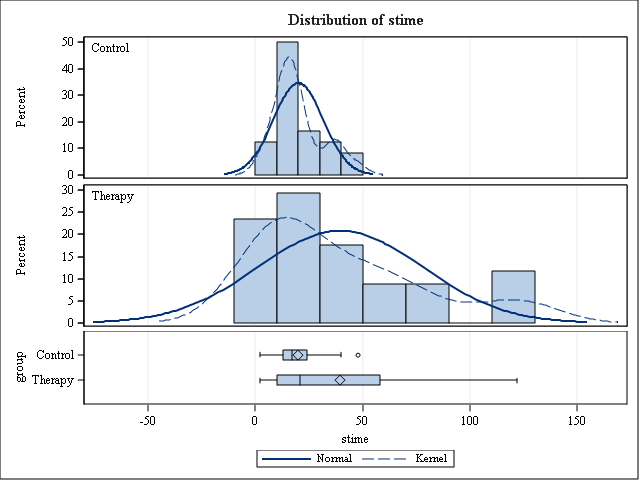
\includegraphics[width = 0.8\textwidth]{diststimes.png}
\end{center}
According to the plots, the distribution of these two groups are not likely to be normal. 

\item The standard deviation of control group $S_{control} = 11.5420$ and the standard deviation of therapy group $S_{therapy} = 38.3803$. We can see $S_{therapy} > 3 S_{control}$, thus there is a significant difference in the variance.

\item
Randomization test. As there is a significant difference in variance and the disribution is not likely to be normal, we do not tend to choose the pooled t-test or t-test using the Satterthwaite approximation. And in the therapy group we can also find some high values, which cannot be reflected in the Wilcoxon sum rank test. Hence we choose to use the randomization test.
\end{enumerate}

	
	\end{enumerate}
	
	\end{document}